\documentclass[research]{BMSTU-IU8}

%\usepackage[utf8]{inputenc}
%\usepackage[T2A]{fontenc}
%\usepackage{tempora}


\usepackage{amssymb}
\usepackage{amsmath}

\usepackage{listingsutf8}
\usepackage{tikz}
\usepackage{caption}
\usepackage{verbatim}
\usepackage{mathrsfs}
\usepackage{bm}
\usepackage{algorithm2e}
% \usepackage[perpage]{footmisc}
\renewcommand{\thefootnote}{ \arabic{footnote})}
\makeatletter
\renewcommand{\@makefntext}[1]{\noindent\makebox[1.8em][r]{\@thefnmark}~#1}
\makeatother


\usetikzlibrary{shapes.geometric, arrows, calc, positioning}

\student{В. Д. Кадыков}
\theme{Методы построения блоков нелинейной подстановки для использования\\в симметричных криптоалгоритмах}
\group{ИУ8-104}
\supervisor{П. Г. Ключарёв}
\studentFullName{Кадыков Василий Дмитриевич}
\profile{19У472}
\speciality{10.05.01 <<Компьютерная безопасность>>}
\specialization{10.05.01\_01 <<Математические методы защиты информации>>}
\supervisorWithDegree{доктор наук, Ключарёв П. Г.}

\researchConsultant{}
\designConsultant{}
\technologicalConsultant{}
\economicsConsultant{}
\lawsConsultant{}
\normController{}

\usepackage{biblatex}

\defbibenvironment{nirs-bibliography}
  {\list
     {\printfield{labelnumber}}
     {\setlength{\leftmargin}{0pt}% устанавливаем отступ слева
      \setlength{\itemindent}{4.0em}% устанавливаем отступ для номера
      \setlength{\parsep}{\parskip}}
     \renewcommand*{\makelabel}[1]{\hss##1}}
  {\endlist}
  {\item}

\makeatletter
% +10mm ко всем сдвигам
\renewcommand*\l@section{\@dottedtocline{0}{10mm}{2em}}
\renewcommand*\l@structure{\@dottedtocline{0}{10mm}{0em}}
\renewcommand*\l@subsection{\@dottedtocline{1}{15mm}{3em}}
\renewcommand*\l@subsubsection{\@dottedtocline{2}{20mm}{4em}}
\renewcommand*\l@paragraph{\@dottedtocline{3}{25mm}{5em}}
\makeatother



\addbibresource{main.bib}

\begin{document}
\SetKwComment{Comment}{/* }{ */}

    %\maketitle
        
    \setcounter{page}{4}
    \abstract

Стрибог и Кузнечик — это симметричные криптографические примитивы, стандартизированные российским ГОСТ. Они используют один и тот же S-блок \(\pi\), процесс генерации которого не был описан его авторами. В предыдущих работах Бирюков, Перрин и Удовенко восстановили два совершенно разных разложения этого S-блока. В этой работе будут пересмотрены их результаты и будет представлено третье разложение S-блока \(\pi\). Оно является примером довольно небольшого семейства \(2m\)-битных подстановок, которое называется TKlog, и которое тесно связана с логарифмами в конечных полях. Его простота и малое количество используемых компонентов позволяют утверждать, что это та структура, которая была намеренно использована разработчиками Стрибога и Кузнечика.

\(2m\)-битные подстановки этого типа обладают очень сильной алгебраической структурой: они отображают мультипликативные смежные классы по группе \(\text{GF}(2^m)^*\) в аддитивные смежные классы по группе \(\text{GF}(2^m)^*\). Более того, функция, связывающая каждый мультипликативный смежный класс с соответствующим аддитивным смежным классом, всегда по сути одна и та же. Насколько известно, в данной работе впервые представлена эта очень сильная алгебраическая структура.

В данной работе также исследуются другие свойства TKlog и показывается, в частности, что S-блок \(\pi\) всегда может быть разложен подобно первому разложению Бирюкова и др., что объясняет связь между двумя предыдущими разложениями. Это также означает, что всегда возможно эффективно реализовать TKlog аппаратно, и что он всегда демонстрирует визуальный шаблон в своей таблице линейных аппроксимаций, аналогичный тому, который присутствует в \(\pi\).

Хотя в рамках данной работы не были найдены атаки, основанные на этих новых результатах, в работе обсуждается влияние этой работы на безопасность Стрибога и Кузнечика. Для этого было представлено новое, более простое представление линейного слоя Стрибога в виде умножения матриц в таком же поле, в каком определена \(\pi\). В этой работе был получент тот факт, что эта матрица взаимодействует нетривиальным образом с разбиениями, сохраняемыми \(\pi\).

    \tableofcontents % Содержание
    
    \newacronym{АНФ}{АНФ}{Алгебраическая нормальная форма.}
\newacronym{S-Box}{S-блок}{Блок нелинейной подстановки.}

    
    \section{ВВЕДЕНИЕ}
Многие симметричные примитивы полагаются на S-блоки как на единственный источник нелинейности, включая AES \cite{AES01}. Такие объекты представляют собой небольшие функции, отображающие \(\mathbb{F}_2^m\) в \(\mathbb{F}_2^n\), которые часто задаются через таблицы поиска. Их выбор имеет решающее значение, поскольку безопасность и эффективность примитива сильно зависят от их свойств. Например, низкая разностная однородность \cite{Nyb94} подразумевает более высокую устойчивость к разностным атакам \cite{BS91a, BS91b}. С другой стороны, существование простого разложения сильно помогает при эффективной поразрядной (bitsliced) или аппаратной реализации \cite{LW14, CDL16}. Таким образом, от разработчиков алгоритмов ожидается, что они предоставят детальное объяснение своего выбора S-блока. Каждый шифр, опубликованный на конференции по криптографии или безопасности, содержит такие объяснения.

Существует два известных S-блока, для которых данная информация не была предоставлена. Первый — это так называемая «F-таблица» Skipjack \cite{US98}, легковесного блочного шифра, разработанного Американским агентством национальной безопасности (АНБ). Второй — это \(\pi\), 8-битная перестановка, использованная в российской стандартной хеш-функции (позднее названной Стрибог \cite{Fed12}) и блочном шифре (позже названном Кузнечик \cite{Fed15}), а также в первой версии кандидата CAESAR — STRIBOBr1 \cite{Saa14} (которая позже изменила свои компоненты на компоненты из Whirlpool \cite{SB15}). Хотя Стрибог и Кузнечик были впервые опубликованы как национальные стандарты в России (ГОСТ), они с тех пор были включены в другие стандарты. Например, оба были включены IETF как RFC 6986 \cite{DD13} и RFC 7801 \cite{Dol16} соответственно. ISO/IEC также в процессе добавления Кузнечика в список стандартных блочных шифров, а именно стандарт 18033-3.

Было обнаружено, что S-блоки могут быть потенциальными средствами для вставки бэкдора в симметричный алгоритм. В 1997 году Раймен и Прениль предложили стратегию генерации S-блока, которая гарантировала существование линейного перехода с высокой вероятностью \cite{RP97}. Идея заключалась в том, что только разработчик будет знать об этой линейной аппроксимации, но это утверждение позже было опровергнуто \cite{WBDY98}. Позже Патерсон разработал вариант DES с бэкдором и измененными S-блоками \cite{Pat99}. Его общий подход был недавно усовершенствован Bannier и др. \cite{BBF16} для построения блочного шифра, который сохраняет разбиение множество открытых текстов независимо от ключа.

В этом контексте криптоаналитики пытались восстановить структуру плохо описанных S-блоков. Первая такая попытка была предпринята в конце 1970-х, вскоре после публикации DES: Хеллман и др. выявили некоторые закономерности в S-блоках этого блочного шифра \cite{HMS76}. Совсем недавно Бирюков и др. разработали новые инструменты для этой цели. Например, статистический анализ разностных и линейных свойств позволил им показать, что S-блок Skipjack обладает большей устойчивостью к линейным атакам \cite{Mat94}, чем ожидалось \cite{BP15}.

Более важным для рассматриваемого случая является то, что они предоставили первую декомпозицию российского S-блока \(\pi\) \cite{BPU16a, BPU16b}. Соответствующая структура работает на двух ветвях, подобно структуре Фейстеля или Мисти. Однако она гораздо более сложна, так как включает умножения в конечных полях \(GF(2^4)\) и мультиплексор. Позже Перрин и Удовенко нашли разложения этой компоненты, основанные на дискретных логарифмах \cite{PU16}. Они сильно отличаются от предыдущей декомпозиции, но остаются несколько неудовлетворительными из-за сложного «арифметического слоя», которую они используют. Их авторы пришли к следующему выводу: «Мы не смогли найти разумные объяснения для использования структуры из любого из наших разложений в качестве S-блока». На самом деле, существование этих новых структур вызвало больше вопросов, чем ответов, хотя они укрепляют идею о том, что \(\pi\) имеет сильную алгебраическую структуру, вряд ли совместимую с утверждениями о случайности разработчиков» \cite{PU16}. В конце концов, Перрин и Удовенко предположили существование «основного разложения», для которого разложения в работах \cite{BPU16a} и \cite{PU16} были бы лишь побочными эффектами.

\textbf{Произведенный вклад.} В данной работе показывается, что предположение, сделанное в \cite{PU16} было верным и представляется то, что называется "главным разложением" (master decomposition). Оно заключается в том, что \(\pi\), S-блок, используемый в последних двух российских стандартах, работает следующим образом:

$$
\begin{cases}\pi(0) & =\kappa(0) \\ \pi\left(\alpha^{0+17 j}\right) & =\kappa(16-j) \\ \pi\left(\alpha^{i+17 j}\right) & =\kappa(16-i) \oplus\left(\alpha^{17}\right)^{s(j)} \text { для } i>0\end{cases}
$$

где \(\alpha\) является корнем примитивного многочлена, определяющего конечное поле \(\text{GF}(2^8)\), \(s\) — это перестановка над элементами из \( \mathbb{Z}/15\mathbb{Z} \), а \(\kappa: \mathbb{F}_2^4 \to \text{GF}(2^8)\) — это аффинная функция, такая что любой элемент \(x \in \text{GF}(2^8)\) может быть записан как \(x = x_4 \oplus \kappa(x_\kappa) \oplus \kappa(0)\), \(x_4 \in \text{GF}(2^4)\) и \(x_\kappa \in \mathbb{F}_2^4\). Также используются операции "$+$" и "$-$" для обозначения целочисленного сложения и вычитания, и "$\oplus$" для сложения в конечном поле.

Далее эта новая струкрура обобщается, позволяя выбирать \(\kappa\) и \(s\) из соответствующих множеств и получается класс перестановок TKlog. Эта новая структура позволяет легко объяснить особое свойство \(\pi\): оно отображает разбиение \(\text{GF}(2^8)\) на мультипликативные смежные классы \(\text{GF}(2^4)^*\) в разбиение \(\text{GF}(2^8)\) на аддитивные смежные классы \(\text{GF}(2^4)^*\). Более того, ограничение \(\pi\) на каждый независимый мультипликативный смежный класс всегда является одной и той же простой функцией. Таким образом, оно не только отображает одно простое разбиение \(\text{GF}(2^8)\) в другое, но и делает это очень простым способом.

В этой работе также доказывается, что такие перестановки всегда могут быть записаны в виде, аналогичном декомпозиции, представленной в \cite{BPU16a}, так что полученная декомпозиция обеспечивает недостающее звено между первой декомпозицией из \cite{BPU16a} и декомпозицией из \cite{PU16}, основанной на логарифмах. С помощью аргументов подсчета показывается, что мощность множества TKlog, работающего с 8 битами, и количество аффинных 8-битных перестановок сравнимы по величине, а значит, вероятность того, что случайная перестановка является элементом множества TKlog, пренебрежимо мала. Следовательно, утверждатся, что наличие этой структуры в \(\pi\) является преднамеренным выбором её разработчиков. Используя экспериментальные аргументы, предлагается простой алгоритм генерации, типичным результатом которого будет \(\pi\).

Наконец, стоит отметить, что линейный блок Streebog является MDS-матрицей с коэффициентами из \(\text{GF}(2^8)\), где примитивный многочлен, используемый для определения представления ее элементов, на самом деле совпадает с тем, что использован для определения \(\pi\) как TKlog. Таким образом, смежные классы, взаимодействующие с \(\pi\), также взаимодействуют с линейным блоком Streebog. В этой работе впервые обсуждаются последствия новой структуры в \(\pi\) с точки зрения безопасности, но их использование в криптоанализе остается в виде открытой проблемы.

\textbf{Структура работы.} В разделе 2 приведены необходимые теоретические сведения, как с точки зрения математики, так и с точки зрения предыдущих результатов. TKlog, его связь с \(\pi\) и свойство сохранения разбиений представлены в Разделе 3. Показано, что TKlog является «недостающим звеном» между \cite{BPU16a} и \cite{PU16}, и в Разделе 4 перечислены несколько следствий этого факта. Затем, в Разделе 5, исследуются последствия того, что \(\pi\) является TKlog, для примитивов более высокого уровня. Также будет представлено новое представление линейного слоя Стрибог, которое может представлять самостоятельный интерес. Наконец, Раздел 6 завершает эту работу.

    \section{Необходимый материал}
\subsection{Обозначения и основные определения}
\textbf{Конечные поля.} Существует, с точностью до изоморфизмов, единственное конечное поле, состоящее из \(2^n\) элементов, которое обозначается \(\text{GF}(2^n)\). В данной работе будет использоваться "\(\oplus\)" для обозначения сложения в поле, а \(a \odot b\) или \(ab\) для обозначения произведения \(a, b \in \text{GF}(2^n)\). Для всех \(x \in \text{GF}(2^n)\) выполняется \(x^{2^n} \oplus x = 0\).

Пусть \(n = 2m\), тогда определим отображение из \(\text{GF}(2^{2m})\) в \(\text{GF}(2^m)\) как функцию \(\text{Tr}_m: \text{GF}(2^{2m}) \rightarrow \text{GF}(2^m)\), такую что \(\text{Tr}_m(x) = x^{2^m} \oplus x\). Для любого \(\beta \in \text{GF}(2^{2m})\), такого что \(\text{Tr}_m(\beta) = 1\), элементы из \(\text{GF}(2^{2m})\) могут быть единственным образом разложены в виде \(a\beta \oplus b\), где \(a\) и \(b\) принадлежат \(\text{GF}(2^m)\). Биекция, отображающая \(x \in \text{GF}(2^{2m})\) в \((a, b) \in \text{GF}(2^m)\)\footnote{Строго говоря, \(GF(2^4)^*\) не является аддитивной подгруппой \(GF(2^8)\). Таким образом, множество \(\{a \oplus x, x \in GF(2^4)^*\}\) формально не является аддитивным смежным классом. Однако, для простоты будем немного злоупотреблять этим термином и называть такие множества "аддитивными смежными классами \(GF(2^4)^*\)".} такая, что \(x = a\beta \oplus b\), обозначается как \(\text{Split}_\beta\), таким образом \(\text{Split}_\beta(a\beta \oplus b) = (a, b)\). Это линейная функция.

Будем использовать \(S^*\) для обозначения множества \(S\) без нуля. Хотя \(\text{GF}(2^m)^*\) не является аддитивной группой, будем называть \(\{a \oplus x, x \in \text{GF}(2^m)^*\}\) аддитивным смежным классом \(\text{GF}(2^m)^*\) для упрощения. Пусть \(S\) — это множество, \(a\) — константа, тогда обозначим \(a \oplus S = \{a \oplus x, x \in S\}\) и \(aS = a \odot S = \{a \odot x, x \in S\}\).

\textbf{Двоичные последовательности как элементы кольца.} Полем \(\text{GF}(2^n)\) называется \(\mathbb{F}_2[X]/p(X)\) для некоторого неприводимого полинома \(p\) степени \(n\). Если \(\alpha\) — это корень \(p\), то все элементы \(\text{GF}(2^n)\) можно представить в виде \(\sum_{i=0}^{n-1} x_i \alpha^i\), где \(x_i \in \mathbb{F}_2\). Тогда двоичную последовательность \((x_0, \ldots, x_{n-1}) \in \mathbb{F}_2^n\) можно представить в виде \(\sum_{i=0}^{n-1} x_i \alpha^i \in \text{GF}(2^n)\) аналогично тому, как ее можно представить в виде \(\sum_{i=0}^{n-1} x_i 2^i \in \mathbb{Z}/2^n\mathbb{Z}\). В этом случае, двоичное представление \(a \oplus b\) для \(a, b \in \text{GF}(2^n)\) является исключающим ИЛИ (XOR) двоичных представлений \(a\) и \(b\).

\textbf{Логарифмы.} Для любого \(x \in \text{GF}(2^n)^*\), логарифм \(\log_\alpha(x)\) — это целое число из \(\mathbb{Z}/(2^n - 1)\mathbb{Z}\) такое, что \(\alpha^{\log_\alpha(x)} = x\). Такая функция не является перестановкой, потому что она не определена в 0. Эта проблема может быть решена различными способами. В \cite{HN10} Хакала и Ниберг изучают функцию, которая в этой работе будет обозначаться как \(\log_{\alpha}^{\text{HN}}\), в то время как Фэнг и др. в \cite{FLY09} предложили другую вариацию, частный случай которой является перестановкой \(\text{GF}(2^n)\), и которая будет обозначаться как \(\log_{\alpha}^{\text{FLY}}\). Эти две функции отображают \(\text{GF}(2^n)\) в \(\mathbb{Z}/2^n\mathbb{Z}\) и определены следующим образом:
$$
\log _\alpha^{\mathrm{HN}}(x)=\left\{\begin{array}{ll}
        2^n-1 & \text { если } x=0, \\
        0 & \text { если } x=1, \\
        \log _\alpha(x) & \text { если } x \notin\{0,1\},
        \end{array} \quad \text { и } \log _\alpha^{\mathrm{FLY}}(x)= \begin{cases}0 & \text { если } x=0 \\
        2^n-1 & \text { если } x=1, \\
        \log _\alpha(x) & \text { если } x \notin\{0,1\} .\end{cases}\right.
$$

\textbf{Булевы функции.} Пусть \( F : \mathbb{F}_2^n \rightarrow \mathbb{F}_2^m \) — функция. Таблица линейных аппроксимаций (LAT) или преобразование Уолша функции \( F \) представляет собой матрицу размером \( 2^n \times 2^m \), обозначаемую как \( \mathcal{W}_F \), для которой:

\[
\mathcal{W}_F(a, b) = \sum_{x \in \mathbb{F}_2^n} (-1)^{a \cdot x \oplus b \cdot F(x)},
\] где \( a \cdot b \) — это обычное скалярное произведение в \(\mathbb{F}_2^n\). Максимальное значение \(|\mathcal{W}_F(a, b)|\) для \(b \neq 0\) называется линейностью \( F \). Таблица распределения разностей (Difference Distribution Table, DDT) функции \( F \) — это матрица \( 2^n \times 2^m \), обозначаемая \(\delta_F\), такая что
\[
\delta_F(a, b) = \# \{ x \in \mathbb{F}_2^n \mid F(x \oplus a) \oplus F(x) = b \}.
\]

Максимальное значение \(\delta_F(a, b)\) для \(a \neq 0\) yfpsdftncz hfpyjcnyjq однородностью \( F \). Если \( A \) и \( B \) — аффинные перестановки над \(\mathbb{F}_2^m\) и \(\mathbb{F}_2^n\) соответственно, то \( F \) аффинно эквивалентна \( G = B \circ F \circ A \). Кроме того, пусть \( L_A \) и \( L_B \) — линейные составляющие \( A \) и \( B \). Тогда LAT функции \( G \) вычисляется как:

\[
\mathcal{W}_G(a, b) = \mathcal{W}_F((L_A^{-1})^T(a), L_B^T(b)).
\]

Аффинно-эквивалентность может быть обобщена в CCZ-эквивалентность \cite{CCZ98}: две функции \( F: \mathbb{F}_2^n \rightarrow \mathbb{F}_2^m \) и \( G: \mathbb{F}_2^n \rightarrow \mathbb{F}_2^m \) являются CCZ-эквивалентными, если существует аффинная перестановка \( \mathcal{A} \) множества \(\mathbb{F}_2^n \times \mathbb{F}_2^m\) такая, что

\[
\{(x, F(x)) \mid x \in \mathbb{F}_2^n \} = \mathcal{A}(\{(x, G(x)) \mid x \in \mathbb{F}_2^n \}).
\]

Эта форма эквивалентности известна тем, что сохраняет, в том числе, разностную однородность и линейность.
    \section{TKlog}

В этом разделе мы вводим новый тип перестановки, который мы называем TKlog, особым случаем которого является \(\pi\). Поскольку Стрибог и Кузнечик были разработаны "ТК-26"\footnote{[Тут сноска о значении ТК-26]}, мы используем буквы "TK" для именования этой структуры. Она обладает логарифмическими свойствами, хотя и отображает \(\mathrm{GF}(2^{2m})\) на себя, а не на \(\mathbb{Z}/2^{2m}\mathbb{Z}\), отсюда и "log" часть имени. Более точно, она отображает разбиение \(\mathrm{GF}(2^{2m})\) на мультипликативные классы \(\mathrm{GF}(2^m)^*\) в её разбиение на аддитивные классы \(\mathrm{GF}(2^m)\), и её ограничение на каждый мультипликативный класс по существу одинаково для всех классов. Мы определяем эту структуру в секции 3.1 и представляем детали этого сохраняющего разбиение свойства в секции 3.2.

\subsection{TKlog Перестановочная Структура}

\textbf{TKlog.} Пусть \(\mathrm{GF}(2^{2m}) = \mathbb{F}_2[X]/p(X)\) — конечное поле чётной степени, определённое примитивным многочленом \(p\). Мультипликативная подгруппа \(\mathrm{GF}(2^{2m})^*\) циклична и генерируется \(\alpha\), такой что \(p(\alpha) = 0\). В этом контексте \(\alpha^{2m+1}\) является генератором мультипликативной подгруппы подполей \(\mathrm{GF}(2^m)\).

\textbf{Определение 1 (TKlog).} TKlog — это перестановка, действующая на \(\mathrm{GF}(2^{2m}) = \mathbb{F}_2[X]/p(X)\) для некоторого примитивного многочлена \(p\) с корнем \(\alpha\). Она параметризована:
\begin{itemize}
    \item аффинной функцией \(\kappa : \mathbb{F}^m_2 \to \mathrm{GF}(2^{2m})\) такой, что любое \(x \in \mathrm{GF}(2^{2m})\) может быть записано как \(x = x_m \oplus \kappa(x_\kappa) \oplus \kappa(0)\) для некоторых \(x_m \in \mathrm{GF}(2^m)\) и \(x_\kappa \in \mathbb{F}^m_2\),\footnote{[Дополнительное пояснение может быть добавлено здесь при необходимости]}
    \item перестановкой \(s\) из \(\mathbb{Z}/(2^m - 1)\mathbb{Z}\).
\end{itemize}
Соответствующий TKlog обозначается \(T_{\kappa,s}\) и действует следующим образом:
% \[
% \begin{cases}
% T_{\kappa,s}(0) = \kappa(0), \
% T_{\kappa,s}((\alpha^{2m+1})^j) = \kappa(2^m - j), & \text{для } 1 \leq j \leq 2^m - 1, \
% T_{\kappa,s}(\alpha^i + (2m+1)j) = \kappa(2^m - i) \oplus (\alpha^{2m+1})^{s(j)}, & \text{для } 0 < i, 0 \leq j < 2^m - 1,
% \end{cases}
% \]
где факт, что \(1 \leq j \leq 2^m - 1\) вместо \(0 \leq j < 2^m - 1\), когда \(x \in \mathrm{GF}(2^m)^*\), происходит из неявного использования логарифма Фэнга и др. Алгоритм 3 (в приложении A9) оценивает такую перестановку.
    \section{Недостающее звено}
Структура TKlog является недостающим звеном между двумя предыдущими разложениями \(\pi\). Ее связь с логарифмическими разложениями \cite{PU16} естественна, так как обе состоят из дискретного логарифма с последующей арифметикой. Тот факт, что \(\pi\) имеет TU-разложение, остается удивительным. В Разделе 3.1 будет показано, что это всегда так для TKlog. В Разделе 3.2 также будут перечислены некоторые следствия этого свойства.

\subsection{TU-разложение всегда существует}
TKlog всегда можно выразить способом, очень похожим на первое разложение Бирюкова и др. \cite{BPU16a}. Для того чтобы установить это, введем следующую лемму:

\textbf{Лемма 2.} Существует функция \(\gamma : (\mathbb{Z}/(2m + 1)\mathbb{Z})^* \to \mathbb{Z}/(2m - 1)\mathbb{Z}\) такая, что 
\[
\{x \in GF(2^{2m}), \mathrm{Tr}(x) = 1\} = \{\alpha^{i + (2m+1)\gamma(i)}, i \in \mathbb{Z}/(2m + 1)Z^*\}.
\]

\begin{proof}
Пусть \((a, b) = \mathrm{Split}_{\beta}(x)\). Если \(x \notin GF(2^m)\), то \(a \neq 0\) и можно записать \(x = a(\beta \oplus c)\), где \(c = b/a\) является элементом \(GF(2^m)\), таким, что \(\mathrm{Tr}(\beta \oplus c) = \mathrm{Tr}(\beta) = 1\). Так как такое разложение существует для всех \(x \notin GF(2^m)\), получается, что множество 
\[
\{\mathrm{log^{FLY}}_{\alpha}(c \oplus \beta), c \in GF(2^m)\}
\]
должно содержать представителя каждого класса эквивалентности по модулю \(2^m + 1\), так как в противном случае некоторые элементы \(\alpha^{i + (2^m+1)j}\) при \(i \neq 0\) не могли бы быть записаны в виде \(a(\beta \oplus c)\).

Тогда \(\{\mathrm{log^{FLY}}_{\alpha}(c \oplus \beta) \mod (2^m + 1), c \in GF(2^m)\} = \{1, \ldots, 2^m\}\),
и, следовательно, должна существовать функция \(\gamma\), представленная выше, такая что:
\[
\{\mathrm{log^{FLY}}_{\alpha}(с \oplus \beta), с \in GF(2^m)\} = \{1 + (2^m + 1)\gamma(1), \ldots, 2^m + (2^m + 1)\gamma(2^m)\}.
\]
\end{proof}

\textbf{Теорема 2}\textit{(TU-разложение TKlog).}
Перестановка \(\mathscr{T}_{\kappa, s}\) над \(GF(2^{2m})\) имеет TU-разложение, включающее три \(m\)-битные подстановки \(\tau, \nu\) и \(\sigma\), и \(m\)-битную функцию \(\phi\). Это представлено в Алгоритме \ref{alg:alg02}.

\begin{algorithm}[htp!]
  \KwData{$x \in \text{GF}(2^8)$}
  $a, b \gets Split_{\beta}(x)$ \Comment*[r]{Входной линейный слой}
  \eIf{$a = 0$} {
    $\ell \gets \tau(b)$;
  }{
    $\ell \gets \nu(b/a)$;
  }
  $h \gets \sigma(\phi(\ell) \odot a)$ \Comment*[r]{$h=U_{T_a(b)}(a)=U_{\ell}(a)$}
  return $k(\ell) \oplus h$ \Comment*[r]{Выходной линейный слой}
\caption{TU-разложение TKlog}
\label{alg:alg02}
\end{algorithm}

\begin{proof}
Пусть \((a, b) = \mathrm{Split}_{\beta}(x)\). Пусть \(a\) будет соответствовать правой ветви TU-разложения, а \(b/a\) левой. Случай \(a = 0\) является особым случаем. Это доказательство является прямым в том смысле, что оно заключается только в правильном определении подкомпонентов \(\tau, \sigma, \nu\) и \(\phi\) и проверке их работы.

$\bm{a=0.}$ Если \(a = 0\), то \(x \in GF(2^m)\), и по определению TKlog получаем \(\mathscr{T}_{\kappa, s}(x) = \kappa(\tau(b))\), где
\[
\tau : 
\begin{cases}
GF(2^m) & \to \mathbb{F}^m_2 \\
0 & \mapsto 0, \\
b & \mapsto 2^m - \mathrm{log^{FLY}}_{(\alpha^{2m+1})}(b), \text{ если } b \neq 0.
\end{cases}
\]

Действительно, пусть \(x = b = \alpha^{(2^m+1)j}\) для \(0 < j \leq 2^m - 1\). Для \(b \neq 0, 1\) получается, что \(\mathrm{log^{FLY}}_{(\alpha^{2^m+1})}(b) = \mathrm{log}_{\alpha}(b)/(2^m + 1) = j\), тогда \(\kappa(\tau(b))\) равно \(\mathscr{T}_{\kappa, s}(x)\). Для \(b = 0\), получаем, что \(\kappa(\tau(b)) = \mathscr{T}_{\kappa, s}(x)\). Для \(b = 1\), \(\mathrm{log^{FLY}}_{\alpha}(b) = 2^{2m} - 1 = (2^m - 1)(2^m + 1)\), тогда \(j = 2^m - 1\), что равно \(\mathrm{log^{FLY}}_{(\alpha^{2^m+1})}(b)\).

$\bm{a \neq 0.}$ В противном случае, для \(a \neq 0\), можно записать \(x = \alpha(\beta \oplus b/a)\) и, поскольку 0 и 1 являются элементами \(GF(2^m)\), получается, что \(x \neq 0, 1\), тогда \(\mathrm{log^{FLY}}_{\alpha}(x) = \mathrm{log}_{\alpha}(x)\). Для оценки \(\mathscr{T}_{\kappa,s}(x)\), необходимо найти \(i\) и \(j\) такие, что \(\alpha(\beta \oplus b/a) = \alpha^{i+(2^m+1)j}\). Получается, что \(\mathrm{Tr}_m(a) = 0\) и \(\mathrm{Tr}_m(\beta \oplus b/a) = 1\), поэтому можно применить Лемму 2, чтобы записать
\begin{equation}
  \begin{cases}
    \beta \oplus b/a & = \alpha^{i+(2^m+1)\gamma(i)} \\
    a & = \alpha^{(2^m+1)(j-\gamma(i))}.
  \end{cases}
  \label{eq:03}
\end{equation}

Определим подстановки \(\nu, \sigma\) и функцию \(\phi\) следующим образом:

\begin{itemize}
  \item Перестановка \(\nu\) отражает то, как логарифм и арифметическая операция \(x \mapsto 2^m - x\) действуют на \(b/a\), чтобы вернуть правильный вход для \(\kappa\):
  \[
  \nu :
  \begin{cases}
  GF(2^m) & \to \mathbb{F}^4_2 \\
  c & \mapsto 2^m - (\mathrm{log}_{\alpha}(\beta \oplus c) \mod (2^m + 1)),
  \end{cases}
  \]
  тогда \(\nu(b/a) = 2^m - i\).

  \item Перестановка \(\sigma\) соответствует подстановке \(s\), примененной к \(j\):
  \[
  \sigma :
  \begin{cases}
  GF(2^m) & \to GF(2^m) \\
  0 & \mapsto 0 \\
  c & \mapsto (\alpha^{2^m+1})^{s(\mathrm{log}_{(\alpha^{2^m+1})}(c))}, \text{ при } c \neq 0.
  \end{cases}
  \]

  \item Функция \(\phi\) соответствует функции \(\gamma\), введенной в Лемме 2:
  \[
  \phi :
  \begin{cases}
  \mathbb{F}^m_2 & \to GF(2^m) \\
  i & \mapsto \alpha^{(2^m+1)\gamma(2^m-i)},
  \end{cases}
  \]
  где \(i \in \mathbb{F}^m_2\) интерпретируется как элемент \(\mathbb{Z}/(2m + 1)\mathbb{Z}\). Стоит заметить, что \(\phi(i) \neq 0\) для любого \(i\). Используя \(\nu(b/a) = 2^m - i\), получается:
  \[
  (\phi \circ \nu)(b/a) = \phi(2^m - i) = \alpha^{(2^m+1)\gamma(i)}
  \]

  и, также используя уравнение~\ref{eq:03}, получаем
  \[
  (\phi \circ \nu)(b/a) \odot \alpha = \alpha^{(2^m+1)\gamma(i)} \odot \alpha^{(2^m+1)(j-\gamma(i))} = \alpha^{(2^m+1)j}.
  \]
\end{itemize}

  Объединяя полученный результат с определением \(\sigma\), получаем
  \[
  \sigma((\phi \circ \nu)(b/a) \odot \alpha) = \sigma(\alpha^{(2^m+1)j}) = (\alpha^{2^m+1})^{s(j)}.
  \]

Тогда можно записать для любого \(a \neq 0\), что
\[
  \mathscr{T}_{\kappa, s}(a \beta \oplus b)=\kappa(\underbrace{\nu(b / a)}_{2^m-i}) \oplus \underbrace{\sigma((\phi \circ \nu)(b / a) \odot a)}_{\left(\alpha^{2^m+1}\right)^{s(j)}} .
\]

Когда \(a = 0\), элемент справа от \(\oplus\) аннулируется, так как \(\sigma(0) = 0\). Поэтому, для случая \(a = 0\), можем записать:
\[
  \mathscr{T}_{\kappa, s}(a \beta \oplus b)=\underbrace{\kappa(\tau(b))}_{\mathscr{T}_{\kappa, s}(b)} \oplus \underbrace{\sigma((\phi \circ \nu)(b / a) \odot a)}_0,
\]
что представляет собой то же выражение, что и в случае \(\alpha \neq 0\), за исключением того, что аргумент \(\kappa\) принимает значение \(\tau(b)\) вместо \(\nu(b/a)\). В результате можно оценить эту функцию в два этапа:

\begin{enumerate}
  \item Пусть \((a, b) = \mathrm{Split}_{\beta}(x)\). Если \(a = 0\), пусть \(\ell = \tau(b)\); иначе пусть \(\ell = \nu(b/a)\).
  \item Вернуть \(\kappa(\ell) \oplus \sigma(\phi(\ell) \cdot \alpha)\).
\end{enumerate}

Этот процесс описан в Алгоритме~\ref{alg:alg02}.
\end{proof}

Существование TU-разложения Бирюкова и др., очевидно, является прямым следствием этой теоремы. Связь между этим разложением и исходной структурой TKlog позволяет лучше понять некоторые закономерности, существующие в этом разложении.

Во-первых, компонент, который Бирюков и др. назвали \(\nu_0\), играет роль \(\tau\) в Теореме 2. Поскольку \(\tau\) по сути является логарифмом с основанием \(\alpha^{-(2m+1)}\), неудивительно, что в \cite{PU16} было отмечено, что \(\nu_0\) аффинно-эквивалентен логарифму.

Во-вторых, линейные слои \(\alpha\) и \(\omega\) исходного разложения по сути разбивают \(GF(2^{2m})\) на \(GF(2^m)^2\), а затем соединяют обратно, отсюда и отношение, представленное в Уравнении~\ref{eq:01}. Кроме того, выходной слой \(\omega\) сложнее входного слоя \(\alpha\), поскольку он также оценивает линейную часть \(\kappa\).

\subsection{Свойства, объясняемые TU-разложением}

\textbf{Эффективная аппаратная реализация.} Знание разложения из Теоремы 2 позволило Бирюкову и др. значительно улучшить реализацию \(\pi\): они сделали схему, реализующую данную подстановку, уменьшив площадь и задержку в 2.5 и 8 раз соответственно \cite{BPU16b}. Можно ожидать аналогичных улучшений для всех 8-битных TKlog.

\textbf{Визуальный артефакт в LAT.} Бирюков и др. использовали особый визуальный артефакт в LAT \(\pi\) для выполнения первого шага своего TU-разложения, а именно наличие столбцов с меньшим количеством различных коэффициентов, чем у других. Они показали, что эта закономерность является прямым следствием структуры, которую они определили в этом S-блоке, а именно структуры из Теоремы 2. Как следствие, можно обобщить их результат на все экземпляры TKlog.

\textbf{Лемма 3.}
Рассмотрим экземпляр TKlog \(\mathscr{T}_{\kappa,\alpha,s}\), пусть \(\text{Split}_{\beta}, \tau, \sigma, \nu\) и \(\phi\) будут подфункциями, используемыми для реализации его TU-разложения, как представлено в Алгоритме 2, и пусть \(\phi_{\kappa} : GF(2^{2m}) \to GF(2^m) \times GF(2^m)\) будет аффинной биекцией вида \(\phi_{\kappa}(\kappa(x) \oplus v) = (x, v)\).

Пусть \(F\) подстановка над \(GF (2^m)^2\), определенная как \(F = \phi_{\kappa} \circ \mathscr{T}_{\kappa,s} \circ \text{Split}^{-1}_{\beta}\), она состоит из TU-разложения \(\mathscr{T}_{\kappa,s}\) без входных и выходных линейных слоев. Тогда, для \((a_L, a_R) \neq (0, 0)\) и \(b_L \neq 0\) получается
\[
\mathcal{W}_{F}[(a_L, a_R), (b_L, 0)] = \left(\mathcal{W}_{\tau}[a_L, b_L] \pm 2^m\right)[a_L \neq 0],
\]
где \([a_L \neq 0] = 0\) при \(a_L = 0\), и \(1\) в противном случае.

Доказательство этой леммы по сути аналогично тому, которое дали Бирюков и др. в расширенной версии своей статьи \cite{BPU16b}. Для полноты изложения, оно будет приведено в Приложении Г. 

Поскольку \(\tau\) по сути является дискретным логарифмом, его нелинейность всегда велика, так что закономерность всегда видна. Действительно, из-за этой высокой нелинейности, \(|\mathcal{W}_{\tau}[a_L, b_L]|\) может принимать значения, значительно меньшие, чем \(2^m\), что означает, что низкий контраст будет всегда присутствовать.

В работе \cite{BPU16a} авторы оригинального разложения отметили, что им повезло, поскольку стечение обстоятельств, которое привело к успеху их разложения, казалось маловероятным. По их собственным словам (страница 19 из \cite{BPU16b}):
\begin{quote}
[Визуальный шаблон] вызван совокупностью трех элементов:
\begin{itemize}
\item использование мультиплексора;
\item использование инверсии в конечном поле;
\item факт того, что \(\nu_0\) обладает хорошей нелинейностью
\end{itemize}
По иронии судьбы, единственная ''неудивительная'' подкомпонента \(\pi\), а именно обратная функция, является одной из причин, по которой нам удалось осуществить реверс-инжиниринг именно этого S-блока. Если бы [инверсия] была заменена на другой (и, возможно, более слабый!) S-блок, не было бы ни одной из строк в LAT, с которых начался бы наш реверс-инжиниринг.
\end{quote}

Теперь видно, что все эти события являются не удачей, а прямым следствиемс структуры TKlog \(\pi\).

Кстати, это отличный метод для выявления такой структуры, если кто-то другой решит использовать ее и попытается скрыть этот факт. В работе \cite{PU16} Перрин и Удовенко предложили построить график дисперсии абсолютного значения коэффициентов в каждой строке/столбце LAT. Они заметили, что для \(\pi\) в некоторых столбцах наблюдается резкое падение. Из Леммы 3 следует, что эта закономерность является неотъемлемым свойством TKlog, которое всегда будет свидетельствовать о наличии такой структуры. Более того, если экземпляр TKlog усложнить (obfuscated), составив его из аффинных слоев, этот шаблон сохранится и фактически даст некоторую информацию о линейной части этих аффинных слоев.

Кроме того, поскольку TKlog всегда имеет TU-разложение, он всегда будет иметь векторное пространство размерности \(n = 2^m\)  внутри множества координат нулей его LAT \cite{CP19}. Это также можно обнаружить, и таким образом выяснить, что экземпляр является TKlog.

\textbf{CCZ-эквивалентность.} Из Теоремы 2 известно, что TKlog всегда аффинно-эквивалентен подстановке \(P : (GF(2^m))^2 \to (\mathbb{F}_2^m)^2\), такой, что
\[
P(b, a) = \left(T_a(b), U_{T_a(b)}(a)\right), \text{ где }\left\{\begin{array}{l}
T_a(b) = \tau(b) \cdot [a = 0] \oplus \nu(b/a) \times [a \neq 0], \\
U_k(a) = \sigma(a/\phi(k)),
\end{array}\right.
\]
где \([a = 0]\) — это булева функция, отображающая \(0\) в \(1\) и \(a \neq 0\) в точке \(0\), и где \([a \neq 0] = 1 \oplus [a = 0]\).

Как объясняется в \cite{CP19}, существование такого разложения, в котором \(T_r\) является подстановкой для всех \(r \in \mathbb{F}_2^m\), эквивалентно возможности так называемого \(m\)-поворота (\(m\)-twist), операции, которая сохраняет класс CCZ-эквивалентности, но априори не сохраняет класс AE-эквивалентности. Поскольку функциональная инверсия также сохраняет класс CCZ-эквивалентности, получается следующее следствие из Теоремы 2.

\textbf{Следствие 3.}
Пусть \(T\) и \(U\) такие, как определено выше. И пусть соответствующий экземпляр TKlog и его инверсия являются CCZ-эквивалентными функции \(F : \mathbb{F}_2^m \times GF(2^m) \to \mathbb{F}_2^m \times GF(2^m)\), такой, что
\[
F(b, a) = \left(T_a^{-1}(b), U_b(a)\right), \text{ где }\left
\{\begin{array}{l}
T_a^{-1}(b) = \tau^{-1}(b) \times [a = 0] \oplus \left(\nu^{-1}(b) \odot a\right) \times [a \neq 0], \\
U_b(a) = \sigma(a/\phi(b)),
\end{array}\right.
\]
\begin{proof}
По определению (\cite{CP19}), \(m\)-поворот отображает функцию \(P : (r, \ell) \mapsto \left(T_r(\ell), U_{T_r(\ell)}(r)\right)\) в \(F : (r, \ell) \mapsto \left(T_r^{-1}(\ell), U_{\ell}(r)\right)\).
\end{proof}

В случае \(\pi\) получилось сгенерировать функцию \(F_\pi\), которая является CCZ-эквивалентной ей, как указано в Следствии 3. Ее таблица поиска представлена в Приложении А (см. Таблицу \ref{tab:A2}). Она имеет Такие же разностные и расширенные спектры Уолша, что и \(\pi\), и, как и \(\pi\), все ее координаты имеют степень 7. Однако это не подстановка: у 15 элементов есть по 3 прообраза, у 75 — по 2, а у оставшихся 61 — по 1.
    \section{Новая информация о российских примитивах}

В этом разделе обсуждаются последствия того факта, что \(\pi\) является экземпляром TKlog. Сначала утверждается, что наличие структуры TKlog может быть осознанным выбором разработчиков (Раздел 4.1). Затем в Раздел 4.2 вводится новое представление двоичной матрицы, которая используется в алгоритме Стрибог, с помощью которого рассматриваются некоторые взаимодействия между разбиениями, сохраняемыми \(\pi\), и этой линейной компонентой. Наконец, в Разделе 4.3. обсуждаются результаты и их последствия.

\subsection{Вероятный процесс проектирования \(\pi\)}
В свете полученных результатов можно получить некоторую информацию о процессе проектирования \(\pi\). Во-первых, устанавливается, что количество экземпляров TKlog крайне мало, а значит, выбор этой структуры был преднамеренным. Затем, используя некоторые экспериментальные результаты, представляется процесс проектирования, который дает результаты, чрезвычайно похожие на \(\pi\).

\textbf{Плотность множества TKlog.} Помимо высокоуровневого алгоритма, 8-битный TKlog полностью определяется тремя компонентами: примитивным многочленом \(p\) степени $8$ (существует $16$ возможных вариантов), аффинной функцией \(\kappa : x \mapsto \Lambda(x) \oplus \kappa(0)\), где двоичная матрица \(\Lambda\) размера \(8 \times 4\) такая, что \(\Lambda(\mathbb{F}_{2}^{4})\) и \(\text{GF}(2^4)\) лежат в \(\text{GF}(2^8)\), и подстановкой \(s\) над \(\mathbb{Z}/15\mathbb{Z}\). Матрица \(\Lambda\) должна быть такой, чтобы ее первый столбец \(\Lambda_0\) не был элементом \(\text{GF}(2^4)\), второй — не был элементом \(\text{GF}(2^4) \cup (\Lambda_0 \oplus \text{GF}(2^4))\) и т. д., всего для этой матрицы существует существует \((2^8 - 2^4)(2^8 - 2^5)(2^8 - 2^6)(2^8 - 2^7) \approx 2^{30.3}\) вариантов. Таким образом, существует около
\[
  \underbrace{16}_{p} \times \underbrace{2^{30.3}}_{\Lambda} \times \underbrace{2^8}_{\kappa(0)} \times \underbrace{15!}_{s} \approx 2^{82.6}
\]
различных экземпляров 8-битных TKlog.

Это число очень мало. Для сравнения, существует всего \(2^8! \approx 2^{1684}\) подстановок на \(\mathbb{F}_2^8\), из которых \(2^8 \times \prod_{i=0}^{7}(2^8 - 2^i) \approx 2^{70.2}\) являются аффинными. Таким образом, число экземпляров TKlog примерно в 4000 раз больше числа аффинных подстановок.

Эти оценки нужны для того, чтобы дать представление о том, насколько мало число экземпляров TKlog. Предполагается, что генератор случайных подстановок, возвращающий аффинную подстановку, будет намеренно генерировать такой объект. Точно так же можно предположить, что процесс генерации, который привел разработчиков Стрибога к выбору \(\pi\), намеренно вернул экземпляр TKlog.

\textbf{Утверждение.} Разработчики \(\pi\) сознательно выбрали эту структуру, учитывая малое число экземпляров TKlog.

\textbf{Экспериментальные результаты.} Насколько хороши разностные и линейные свойства экземпляров TKlog по сравнению с теми, которые ожидаются от случайной подстановки? Ответ на этот вопрос будет основыватся на анализе S-блока Skipjack из \cite{BP15}, также будут введены следующие понятия.

\textbf{Определение 2} \textit{(Аномалия S-блока.)} Пусть \(F : \mathbb{F}_2^n \to \mathbb{F}_2^n\) — подстановка, \(u(F)\) — ее разностная однородность, а \(N_k(F)\) — число вхождений \(k\) в ее DDT. Разностная аномалия (differential anomaly) \(F\) равна
\[
A_d^F = -\log_2(\mathrm{Pr}[u(G) \leq u(F) \text{ и } N_{u(F)}(G) \leq N_{u(F)}(F)]),
\]
где вероятность берется по всем подстановкам \(G\). Если \(\ell(F)\) — линейность \(F\) и \(N'_k(F)\) — сумма числа вхождений \(k\) и \(-k\) в LAT \(F\), то линейная аномалия (linear anomaly) \(F\) равна
\[
A_\ell^F = -\log_2(\mathrm{Pr}[\ell(G) \leq \ell(F) \text{ и } N'_{\ell(F)}(G) \leq N'_{\ell(F)}(F)]),
\]
где вероятность берется по всем подстановкам \(G\).

S-блок с разностной аномалией, близкой к 0, имеет разностные свойства, близкие свойству случайного S-блока или даже хуже. Разностная аномалия ведет себя так, как и ожидалось: при уменьшении значения разностной однородности ниже ожидаемого, значение аномалии возрастает. Поскольку она содержит больше информации, чем разностная однородность, она позволяет сравнивать S-блоки, для которых это значение одинаково. С криптографической точки зрения, чем выше аномалия, тем лучше, так как это означает, что S-блок обеспечит лучшую защиту от разностных атак. То же самое можно сказать о линейной аномалии.

В своей работе \cite{BP15} Бирюков и Перрин предоставили формулы для вычисления разностных и линейных аномалий, основанные на статистическом распределении коэффициентов DDT и LAT, представленных в \cite{DR07}. Они также показали, что линейная аномалия S-блока Skipjack равна 55.4, так что этот компонент не мог быть сгенерирован случайным образом.

Чтобы попытаться собрать больше информации о процессе проектирования \(\pi\), было сгенерировано \(10^6\) случайных 8-битных экземпляров TKlog. Были изображены разностные и линейные аномалии каждого из них на двумерной диаграмме, представленной на Рисунке \ref{fig:fig03}. Каждому экземпляру соответствует светло-серая точка; более темные точки получаются, когда несколько экземпляров имеют одни и те же разностные и линейные аномалии. Также в эту диаграмму были включены аномалии \(\pi\), \(\log^{\text{FLY}}_\alpha\) и \(\log^{\text{HN}}_\alpha\).

\begin{figure}
  \centering
  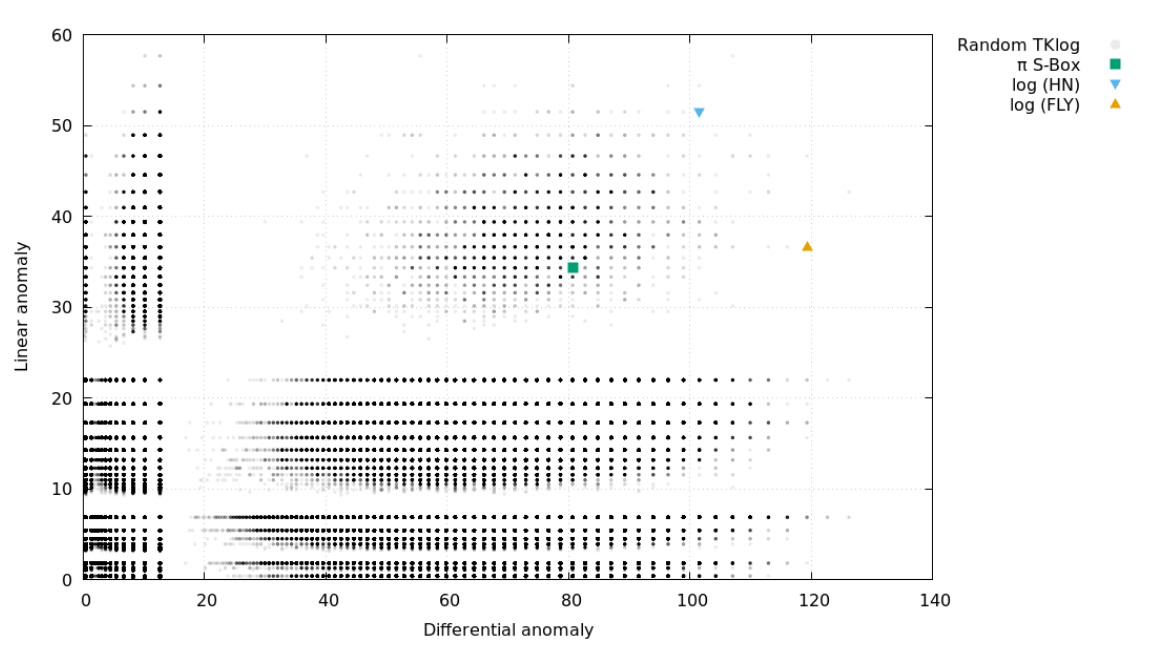
\includegraphics[scale=0.7]{contents/pics/anomalies.png}
  \caption{Разностные и линейные аномалии случайных 8-битных экземпляров TKlog, \(\pi\), \(\log^{\text{FLY}}_\alpha\) и \(\log^{\text{HN}}_\alpha\)}
  \label{fig:fig03}
\end{figure}

Можно заметить, что разностные и линейные аномалии \(\pi\) ''несколько хороши'', но не исключительны относительно аномалий случайного экземпляра TKlog. Точнее, 8-битный TKlog имеет как разностные и линейные аномалии, не ниже, чем у \(\pi\) с вероятностью около \(2^{-10.6}\), и нетрудно получить гораздо лучшие случаи. Они также ниже, чем у \(\log^{\text{FLY}}_\alpha\) и \(\log^{\text{HN}}_\alpha\).

Однако, ни один из полученных случайных экземпляров не имеет лучшей разностной однородности или линейности, чем \(\pi\) (включая \(\log^{\text{FLY}}_\alpha\) и \(\log^{\text{HN}}_\alpha\)). Более того, \(\pi\) находится в области на Рисунке \ref{fig:fig03}, которая содержит большинство экземпляров с той же разностной однородностью и линейностью. Таким образом, аномалии \(\pi\) соответствуют аномалиям случайного экземпляра TKlog с той же разностной однородностью и линейностью.

\textbf{Схема процесса проектирования.} В свете вышеприведенных экспериментальных результатов, можно увидеть, что следующий процесс проектирования приведет к результату, очень похожему на \(\pi\).

\begin{enumerate}
  \item Определить, что наилучшая возможная разностная однородность для 8-битного экземпляра TKlog равна 8, а наилучшая линейность — 56, например, с помощью обширного компьютерного моделирования.
  \item Выбрать случайным образом экземпляр TKlog среди тех, которые обладают указанными выше разностной однородностью и линейностью, не принимая во внимание аномалию.
\end{enumerate}

Эта стратегия естественна до тех пор, пока существует причина навязывать использование TKlog (хотя не получается придумать ни одной). Поскольку  разностные и линейные аномалии \(\pi\) уступают аномалиям \(\log^{\text{FLY}}_\alpha\) и \(\log^{\text{HN}}_\alpha\), целью использования TKlog в данном случае не может быть улучшение криптографических свойств дискретного логарифма. Более того, сильные алгебраические свойства компонентов, описанных в Разделе 2.2, априори требуют осторожности, тем более в случае Стрибога. Действительно, как будет объяснено ниже, его линейный слой нетривиальным образом взаимодействует с соответствующими разбиениями.

\subsection{О линейном слое в Стрибоге}
Бинарная матрица, соответствующая операции L Стрибога, представлена на Рисунке \ref{fig:04}, где черный пиксель соответствует 1, а белый — 0.

\begin{figure}
  \centering
  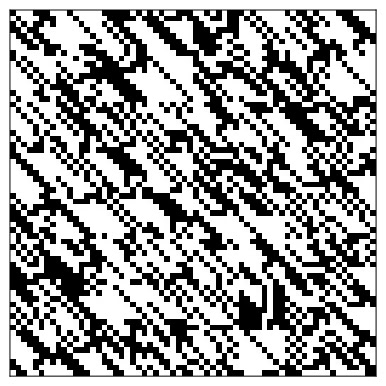
\includegraphics[scale=0.9]{contents/pics/Streebog_matrix.png}
  \caption{Двоичная матрица L \(64 \times 64\), используемая в алгоритме Стрибог}
  \label{fig:04}
\end{figure}

Как можно заметить, матрица имеет сильную структуру. В \cite{KK13} Казимиров и Казимирова показали, что ее можно записать как композицию:
\begin{itemize}
    \item слой 8-битных линейных подстановок \(\ell\), который просто инвертирует порядок битов в каждом байте;
    \item умножение на $8 \times 8$ MDS-матрицу из $GF(2^8) = F_2[X]/P_{KK}(X)$, где \(P_{KK}(X) = X^8 \oplus X^6 \oplus X^5 \oplus X^4 \oplus 1\) — примитивный многочлен степени 8;
    \item величина, обратная слою \(\ell\).
\end{itemize}

В данной работе использовался прямой подход для упрощения этой структуры: каждый байт в строке устанавливался равным 1 по очереди, умножая его на L, затем записывались байты как элементы $GF(2^8) = F_2[X]/p_{\text{min}}(X)$, генерируя матрицу $L^F$ такую следующего вида:
\begin{figure}
  \centering
  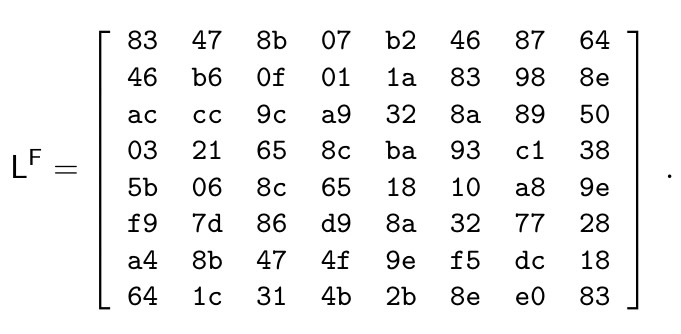
\includegraphics[scale=0.9]{contents/pics/LF_matrix.png}
\end{figure}

Многочлен, используемый Казимировым и Казимировой, является обратным \(p_{\text{min}}\), т.е. \(P_{KK}(1/X) = p_{\text{min}}(X)/X^8\). Оглядываясь назад, очевидно, что, используя этот многочлен, можно устранить обратный порядок бит в байте в представлении ими линейного слоя.

В итоге, если обозначить как $A$ матрицу размера $8 \times 8$, состоящую из элементов из $GF(2^8)$, соответствующую внутреннему состоянию Стрибога, и как $P$ транспонированную матрицу $A$ (как указано в спецификации Стрибог), то применение всей линейной части раундовой функции Стрибог можно записать в виде
\[
(L \circ P)(A) = A^T \times L^F,
\]
где ''$\times$'' обозначает обычное умножение матриц.

\textbf{Аддитивные и мультипликативные смежные классы.} Группа $GF(2^4)^*$ имеет особую связь с $L$. Действительно, применение умножения матрицы Стрибога к вектору \(x_i = [0, \ldots, 0, x, 0, \ldots, 0]\) из $GF(2^8)^8$, так, что \(x_i^i = x\) и \(x_i^k = 0\), при \(k \neq i\), эквивалентно вычислению
\[
v = x^i \times L^F = [L^F_{i,0} \odot x, ..., L^F_{i,7} \odot x],
\]
так, что если \(x \in GF(2^m)^*\), то \(v_j \in LF_{i,j} \cdot GF(2^m)^*\), т.е., оно отображает подполе на его мультипликативные смежные классы. Однако, непонятно, что происходит, когда активны несколько ячеек входного вектора.

\textbf{Кузнечик.} Линейный слой Кузнечика определяется как LFSR с $16$ ячейками, каждая из которых является элементом $GF(2^8)$, и который сдвигается на $16$ тактов. Его также можно представить как умножение на матрицу размером $16 \times 16$. Однако, для представления элементов поля используется другой многочлен, а именно \(p_{\text{kuz}}(X) = X^8 \oplus X^7 \oplus X^6 \oplus X \oplus 1\). Если \(p_{\text{min}}(X) = X^8 \oplus X^4 \oplus X^3 \oplus X^2 \oplus 1\) является первым примитивным многочленом степени $8$, записанным в лексикографическом порядке, то \(p_{\text{kuz}}\) — последний такой многочлен веса $5$, как указано в \cite{LN97}.

В отличие от умножения на матрицу в Стрибоге, в Кузнечике его нельзя записать как матричное умножение в $F_2[X]/p_{\text{min}}(X)$, так что распространение классов смежности, описанное выше для хеш-функции, не применимо к блочному шифру.

\subsection{Обсуждение}

Последствия сохранения разбиения на смежные классы \(\pi\) и его нетривиального взаимодействия с линейным слоем оценить сложно.

В литературе можно найти другие S-блоки, отображающие смежные классы в смежные классы. Например, мономы отображают мультипликативные смежные классы подполя в мультипликативные смежные классы подполя: если \(F: x \mapsto x^d\) является подстановкой на $GF(2^{2m})$, то
\[
F(\alpha^i \cdot GF(2^m)) = \alpha^{d \times i} \odot GF(2^m).
\]

Если убрать их аффинные компоненты, то S-блоки AES \cite{AES01} и Misty1 \cite{Mat97} (среди многих других) демонстрируют такое поведение. Тем не менее, несмотря на их появление в некоторых очень известных целях, мультипликативные смежные классы никогда не использовались в симметричном криптоанализе. Стоит заметить, что разработчики алгоритмов всегда сочетают обратные функции с несвязанными аффинными слоями, чтобы разрушить его алгебраическую структуру. Это консервативное решение, вероятно, предназначено для предотвращения использования мультипликативных смежных классов атак на эти шифры на практике.

Это не так с аддитивными смежными классами. На самом деле, авторы работы \cite{BBF16} намеренно построили S-блок, отображающий аддитивные смежные классы в аддитивные смежные классы, с явной целью использовать этот шаблон в качестве бэкдора. Они показывают, что такое разбиение может быть сохранено при тщательном выборе линейного слоя и может сохраняться в течение произвольного количества раундов. Причина, по которой Bannier и другие рассматривали аддитивные смежные классы, заключается в следующем наблюдении.

\textit{Примечание 1.} Если \(F_k: x \mapsto x \oplus k\) — добавление ключа в $F^n_2$, и \(V\) — векторное подпространство $F^n_2$, тогда
\[
F_k(c \oplus V) = (k \oplus c) \oplus V,
\]
так, что разбиение $F^n_2$ на аддитивные смежные классы \(V\) сохраняется под действием \(F_k\) независимо от \(k\).

В шифре Bannier и др., ключевое расписание может быть произвольно сложным, не препятствуя работе бэкдора. Это свойство не распространяется на разбиение на мультипликативные смежные классы.

Единственным случай (кроме TKlog), когда разбиение на смежные классы отображается на другое разбиение, являются дискретные логарифмы. Действительно, логарифм типа Hakala-Nyberg, действующий на $GF(2^{2m})$, который отображает \(\alpha^{2^m-1}\) в $0$, всегда отображает мультипликативные смежные классы подполя на аддитивные смежные классы $\mathbb{Z}/(2^m - 1)\mathbb{Z}$. В этом случае умножение производится в конечном поле, а сложение с целыми числами. Поскольку эти две операции совершенно разные, маловероятно, что эта характеристика помогает в криптоанализе.

В итоге, рассматривая влияние смежных классов на симметричные примитивы, получается одна из следующих ситуаций:
\begin{enumerate}
    \item разбиение на смежные классы не может быть итеративным, поскольку входное и выходное разбиения находятся в совершенно разных структурах (случай логарифма);
    \item хотя S-блок и линейный слой определены над схожими структурами, была добавлена небольшая функция с явной целью нарушить это сходство (случай AES и аффинной подстановки, использованной в S-блоке);
    \item S-блок и линейный слой были выбраны с выровненными структурами, которые сохраняют одно и то же разбиение, чтобы целенаправленно внедрить бэкдор в блочном шифре \cite{BBF16}.
\end{enumerate}

По-видимому, Кузнечик относится ко второму случаю. Несмотря на то, что разработчики не предоставили свой анализа безопасности, было бы логично, чтобы они выбрали многочлен, используемый для определения конечного поля, в котором функционирует линейный слой, чтобы не 'выравнивать' его со структурой, используемой для построения \(\pi\).

Однако Стрибог не подпадает ни в одну из этих категорий. Входные и выходные смежные классы определены над той же структурой (конечным полем), поэтому он не относится к первой ситуации. S-блок мог быть составлен с аффинным слоем, нарушающим связь с $GF(2^8)$ (как в AES), или линейный слой мог быть определен над другим конечным полем (как в Кузнечике), но ни того, ни другого не происходит, поэтому он не подпадает и под вторую категорию. Тем не менее, хотя линейный слой определен над той же структурой, что и смежные классы, сохраняемые S-блоком, эти разбиения отличаются, и неясно, как они могут взаимодействовать с матричным умножением. Поэтому не является очевидным тот факт, что Стрибог относится к третьей категории, и следующая проблема остается открытой.

\textbf{Открытая проблема 1.} Существует ли способ использовать сохранение разбиения \(\pi\) для атаки на Стрибог?
    \section{Заключение}
В рамках данной работы удалось извлечь новую структуру из \(\pi\), которая, как утверждается в этой работе, была изначально задуманна ее разработчиками. Ее обобщение, TKlog, получается путем композиции дискретного логарифма с простым арифметическим слоем. TKlog объясняет оба предыдущих разложения \(\pi\), таким образом обеспечивая недостающее звено между этими двумя результатами.

Знание об этом разложении позволило объяснить очень специфическое свойство сохранения разбиения \(\pi\). Удивительно, но также было найдено новое представление линейного слоя Стрибога, выраженное в том же конечном поле что и \(\pi\). Хотя пока не получается использовать эти свойства для атаки на эту хеш-функцию, ставится под сомнение вопрос уместности этого решения. Действительно, при работе с компонентами, определенными над идентичными математическими структурами, академические разработчики нарушают это соответствие, например, составляя S-блоки с несвязанными аффинными подстановками. Нужно было более осторожно поступить и в случае Стрибога.

    
    \printbibliography[env=nirs-bibliography]

    \appendix
    \appendixsection{Таблицы поиска}

S-блок $\pi$ был задан только через его таблицу поиска. Она приведена в Таблице \ref{tab:A1}. Функция $F_{\pi}$ получена из $\pi$ из Следствия 3. Ее таблица поиска приведена в Таблице \ref{tab:A2}.

\begin{table}
        \small
        \centering
        \begin{tabular}{c|cccccccccccccccc}
                & .0 & .1 & .2 & .3 & .4 & .5 & .6 & .7 & .8 & .9 & .A & .B & .C & .D & .E & .F \\ \hline
        0. & FC & EE & DD & 11 & CF & 6E & 31 & 16 & FB & C4 & FA & DA & 23 & C5 & 04 & 4D \\
        1. & E9 & 77 & F0 & DB & 93 & 2E & 99 & BA & 17 & 36 & F1 & BB & 14 & CD & 5F & C1 \\
        2. & F9 & 18 & 65 & 5A & E2 & 5C & EF & 21 & 81 & 1C & 3C & 42 & 8B & 01 & 8E & 4F \\
        3. & 05 & 84 & 02 & AE & E3 & 6A & 8F & A0 & 06 & 0B & ED & 98 & 7F & D4 & D3 & 1F \\
        4. & EB & 34 & 2C & 51 & EA & C8 & 48 & AB & F2 & 2A & 68 & A2 & FD & 3A & CE & CC \\
        5. & B5 & 70 & 0E & 56 & 08 & 0C & 76 & 12 & BF & 72 & 13 & 47 & 9C & B7 & 5D & 87 \\
        6. & 15 & A1 & 96 & 29 & 10 & 7B & 9A & C7 & F3 & 91 & 78 & 6F & 9D & 9E & B2 & B1 \\
        7. & 32 & 75 & 19 & 3D & FF & 35 & 8A & 7E & 6D & 54 & C6 & 80 & C3 & BD & 0D & 57 \\
        8. & DF & F5 & 24 & A9 & 3E & A8 & 43 & C9 & D7 & 79 & D6 & F6 & 7C & 22 & B9 & 03 \\
        9. & E0 & 0F & EC & DE & 7A & 94 & B0 & BC & DC & E8 & 28 & 50 & 4E & 33 & 0A & 4A \\
        A. & A7 & 97 & 60 & 73 & 1E & 00 & 62 & 44 & 1A & B8 & 38 & 82 & 64 & 9F & 26 & 41 \\
        B. & AD & 45 & 46 & 92 & 27 & 5E & 55 & 2F & 8C & A3 & A5 & 7D & 69 & D5 & 95 & 3B \\
        C. & 07 & 58 & B3 & 40 & 86 & AC & 1D & F7 & 30 & 37 & 6B & E4 & 88 & D9 & E7 & 89 \\
        D. & E1 & 1B & 83 & 49 & 4C & 3F & F8 & FE & 8D & 53 & AA & 90 & CA & D8 & 85 & 61 \\
        E. & 20 & 71 & 67 & A4 & 2D & 2B & 09 & 5B & CB & 9B & 25 & D0 & BE & E5 & 6C & 52 \\
        F. & 59 & A6 & 74 & D2 & E6 & F4 & B4 & C0 & D1 & 66 & AF & C2 & 39 & 4B & 63 & B6 \\
        \end{tabular}
        \caption{Таблица поиска для \(\pi\). Например, \(\pi(7A)=C6\)}
        \label{tab:A1}
\end{table}

\begin{table}
        \small
        \centering
        \begin{tabular}{c|cccccccccccccccc}
            & .0 & .1 & .2 & .3 & .4 & .5 & .6 & .7 & .8 & .9 & .A & .B & .C & .D & .E & .F  \\ \hline
            0. & 8C & 42 & 87 & C8 & 9E & DF & 13 & 54 & B6 & FB & 3D & 75 & 29 & 60 & AA & E1 \\
            1. & BC & 70 & E8 & 9A & 53 & 25 & BF & C6 & A9 & D2 & 41 & 37 & FD & 84 & 1B & 6E \\
            2. & 0C & D2 & 37 & E8 & 6E & BF & 53 & 84 & C6 & 1B & FD & 25 & A9 & 70 & 9A & 41 \\
            3. & 2C & E3 & 59 & BD & A2 & 44 & F0 & 15 & D7 & 3E & 8A & 66 & 78 & 9F & 21 & CB \\
            4. & 9C & 8F & 9D & 11 & B0 & 36 & 24 & A7 & F8 & 73 & 6B & E9 & 4A & C5 & DE & 52 \\
            5. & 1C & 98 & B3 & 2F & F9 & 61 & 4D & DB & 72 & E7 & C4 & 5E & 80 & 1A & 35 & A6 \\
            6. & 4C & 1D & 20 & 34 & 48 & 5B & 6A & 7E & 83 & 99 & A5 & B2 & CF & D1 & E6 & F7 \\
            7. & FC & 0F & 0D & 01 & 00 & 06 & 04 & 07 & 08 & 03 & 0B & 09 & 0A & 05 & 0E & 02 \\
            8. & CC & 6A & CF & A5 & 1D & 7E & D1 & B2 & 20 & 48 & E6 & 83 & 34 & 5B & F7 & 99 \\
            9. & 5C & 34 & 6A & 5B & CF & F7 & A5 & 99 & 1D & 20 & 7E & 48 & D1 & E6 & B2 & 83 \\
            A. & 7C & FB & 75 & 87 & E1 & 13 & 9E & 60 & 54 & AA & 29 & DF & B6 & 42 & C8 & 3D \\
            B. & 3C & A3 & D9 & 7D & 32 & 94 & E0 & 45 & 67 & CE & BA & 16 & 58 & FF & 81 & 2B \\
            C. & EC & 26 & 4B & 62 & 85 & A8 & C7 & ED & 91 & B4 & D3 & FA & 1E & 39 & 50 & 7F \\
            D. & DC & C4 & 1A & DB & 2F & E7 & 35 & F9 & 4D & 80 & 5E & 98 & 61 & A6 & 72 & B3 \\
            E. & 6C & BA & FF & 45 & 7D & CE & 81 & 32 & E0 & 58 & 16 & A3 & 94 & 2B & 67 & D9 \\
            F. & AC & 52 & A7 & F8 & DE & 8F & 73 & 24 & 36 & 6B & 9D & C5 & E9 & B0 & 4A & 11 \\
        \end{tabular}
        \caption{Таблица поиска для $F_{\pi}$, функция CCZ-эквивалентна \(\pi\)}
        \label{tab:A2}
\end{table}
    




    \appendixsection{Алгоритмы}

Алгоритм, реализцющий TKlog, приведен в Алгоритме \ref{alg:algB1}, а алгоритм, рассчитывающий его обратную величину TKexp в Алгоритме \ref{alg:algB2}.

\begin{algorithm}[htp!]
  \KwData{$x \in \text{GF}(2^{2m})$}
  $k \gets \log^{FLY}_\alpha(x)$\;
  \eIf{$k = 0$}{ 
    \Return{$0$} \Comment*[r]{Случай $x = 0$}
  }{
    $i \gets k \mod (2^m + 1)$\;
    $j \gets \left\lfloor k / (2^m + 1) \right\rfloor$ \Comment*[r]{$x = \alpha^{i + (2^m+1)j}$}
    \eIf{$i = 0$}{ 
      \Return{$\kappa(2^m - j)$} \Comment*[r]{т.к. $i = 0$, $j \in \{1, \ldots, 2^m - 1\} = (\mathbb{F}_2^m)^*$}
    }{
      \Return{$\kappa(2^m - i) \oplus \alpha^{(2^m+1)s(j)}$} \Comment*[r]{$i \neq 0$, поэтому $(2^m - i) \in \mathbb{F}_2^m$}
    }
  }
\caption{Перестановка TKlog}
\label{alg:algB1}
\end{algorithm}

\begin{algorithm}[htp!]
  \KwData{$x \in GF(2^{2m})$}
  \eIf{$x = 0$}{
    \Return $0$\;
  }{
    $(k, v) \gets \Phi_{\kappa}(x)$\;
    \eIf{$v = 0$ \Comment*[r]{Случай $x \in \kappa(F^m_2)$}}{
      \Return $\alpha^{(2^m+1)(2^m-k)}$\;
    }{
      $j \gets \log_{\alpha}^{\text{FLY}}(v)/(2^m+1)$ \Comment*[r]{Всегда целое, т.к. $(\alpha^{2^m+1})^j = v$}
      \Return $\alpha^{2^m-k+(2^m+1)s^{-1}(j)}$ \Comment*[r]{$k \in F^m_2$ so $k + 1 \in \{1, \ldots, 2^m\}$}
    }
  }
  \caption{Перестановка TKexp}
  \label{alg:algB2}
\end{algorithm}
    \appendixsection{Нахождение TKlog в \(\pi\)}

Предположение насчет общей структуры TKlog появилось благодаря наблюдениям за TU-разложением Бирюкова и др.

На Рисунке \ref{fig:figC01} показано TU-разложение $\pi$ и описанные ниже обозначения. Для каждого входа $c$ из $\nu_{1}$, то есть для всех $c \in \mathbb{F}_{2}^{4}$, можно определить два множества $A_{c}$ и $B_{c}$ как
$$
\begin{aligned}
& A_{c}=\left\{\alpha^{-1}(x, x \odot \mathcal{I}(c)), \forall x \in \mathbb{F}_{2}^{4}\right\}, \\
& B_{c}=\left\{\omega\left(\nu_{1}(c), y\right), \forall y \in \mathbb{F}_{2}^{4}\right\} .
\end{aligned}
$$
Множества $A_{c}$ являются векторными пространствами, а множества $B_{c}$ - аддитивные смежные классы векторного пространства $\left\{\omega(0, y), \forall y \in \mathbb{F}_{2}^{4}\right\}$.

\begin{figure}
        \centering
        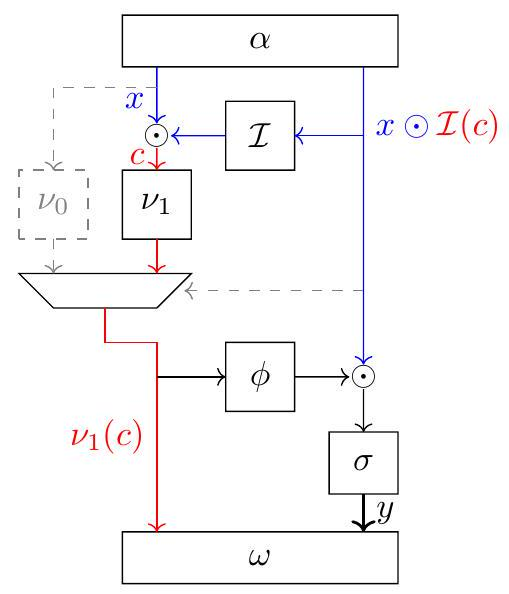
\includegraphics[scale=0.5]{contents/pics/C_pi.jpg}
        \caption{Распространение определенных векторных пространств через \(\pi\)}
        \label{fig:figC01}
\end{figure}

Как видно на Рисунке \ref{fig:figC01}, если применить $\pi$ ко всем элементам $A_{c}$, то получится 16 элементов, из которых 15 принадлежат $B_{c}$. Кроме того, как из Уравнения \eqref{eq:01} следует, что $\left\{\alpha^{-1}(x, 0), \forall x \in \mathbb{F}_{2}^{4}\right\}=\left\{\omega(0, x), \forall x \in \mathbb{F}_{2}^{4}\right\}$. Тогда получается, что
$$
B_{c}=\omega\left(\nu_{1}(c), 0\right) \oplus A_{0}
$$
и что $A_{c}$ каким-то образом связано с $A_{0}$ при помощи умножения в конечном поле. Также можно заметить, что эти множества имеют особую связь с матричным умножением, которое используется в Стрибоге. Пусть L - двоичная матрица $64 \times 64$, используемая в Стрибоге, и пусть $[a, 0, \ldots, 0] \times \mathrm{L}=\left[a_{0}^{\prime}, \ldots, a_{7}^{\prime}\right]$. Если $a$ принимает все значения из $A_{c}$ для некоторого $c \in \mathbb{F}_{2}^{4}$, то $a_{i}^{\prime}$ принимает все значения из $A_{c_{i}}$ для некоторого $c_{i}$. Это свойство выполняется независимо от положения $a$ в изначальном векторе. Поскольку из работы Казимрова и Казимровой \cite{KK13} изместно, что L как-то связана с MDS-матрицей с коэффициентами из $\mathrm{GF}\left(2^{8}\right)$, было получено, что множества $A_{c}$ должны иметь определенную связь с этим полем.

Эти наблюдения в сочетании с тем фактом, что $\pi$ каким-то образом связано с логарифмом \cite{PU16}, позволяют сделать предположение, что векторные пространства $A_{c}$ и аффинные пространства $B_{c}$ на самом деле являются соответственно мультипликативными и аддитивными смежными классами единственного векторного пространства размерности 4, которое было быстро определено как подполе.

Эта догадка позволяет написать первое очень грубое разложение $\pi$, которое в дальнейшем итеративно улучшалось путем переписывания его слагаемых все более простыми способами. Конечным результатом этого долгого и утомительного процесса стало разложение $\pi$ в виде TKlog, которое затем было обобщено.
    \appendixsection{Доказательство Леммы 3}

Следующее доказательство по сути совпадает с доказательством из \cite{BPU16b}, оно приводится только для полноты.

\begin{proof}
Рассмотрим $F=\Phi_{\kappa} \circ \mathscr{T}_{\kappa, h, g_{m}, s} \circ Split_{\beta}^{-1}$. Пусть $a_{L}, a_{R}$ и $b_{L} \neq 0$ — некоторые $m$-битные линейные маски. По определению $LAT$ и $F$ получается:
$$
\begin{aligned}
& \mathcal{W}_{F}\left[a_{L} \| a_{R}, b_{L}| | 0\right] \\
& =\sum_{r \in \operatorname{GF}\left(2^{m}\right)} \sum_{\ell \in \mathrm{GF}\left(2^{m}\right)}(-1)^{a_{L} \cdot \ell+a_{R} \cdot r+\left(b_{L} \| 0\right) \cdot F(r \| \ell)} \\
& =\underbrace{\sum_{\ell \in \mathrm{GF}\left(2^{m}\right)}(-1)^{a_{L} \cdot \ell+b_{L} \cdot \tau(\ell)}}_{r=0}+\sum_{r \in \mathrm{GF}\left(2^{m}\right)^*} \sum_{\ell \in \mathrm{GF}\left(2^{m}\right)}(-1)^{a_{L} \cdot \ell+a_{R} \cdot r+b_{L} \cdot \nu(\ell / r)} .
\end{aligned}
$$
Первая сумма, соответствующая $r=0$, равна $\mathcal{W}_{\tau}\left[a_{L}, b_{L}\right]$. Чтобы оценить вторую сумму (где $r \neq 0$), подставим $u=\nu(\ell / r)$ так, чтобы $\ell=r \odot \nu^{-1}(u)$. Тогда можно записать
$$
\begin{aligned}
& \sum_{r \in \operatorname{GF}\left(2^{m}\right)^{*}} \sum_{u \in \mathrm{GF}\left(2^{m}\right)}(-1)^{a_{L} \cdot\left(r \odot \nu^{-1}(u)\right)+a_{R} \cdot r+b_{L} \cdot u} \\
= & \sum_{u \in \operatorname{GF}\left(2^{m}\right)}(-1)^{b_{L} \cdot u}\bigg(\sum_{r \in \mathrm{GF}\left(2^{m}\right)}(-1)^{a_{L} \cdot\left(r \odot \nu^{-1}(u)\right)+a_{R} \cdot r}-\underbrace{1}_{r=0}\bigg) \\
= & \sum_{u \in \operatorname{GF}\left(2^{m}\right)}(-1)^{b_{L} \cdot u} \sum_{r \in \mathrm{GF}\left(2^{m}\right)}(-1)^{a_{L} \cdot\left(r \odot \nu^{-1}(u)\right)+a_{R} \cdot r}-\underbrace{\sum_{u \in \mathrm{GF}\left(2^{m}\right)}(-1)^{b_{L} \cdot u}}_{=0}
\end{aligned}
$$
Сумма по $r$ соответствует оценке коэффициента Уолша линейной функции, такой, что $r \mapsto r \times \nu^{-1}(u)$. Как следствие, коэффициент равен 0 тогда и только тогда, когда функция $r \mapsto a_{R} \cdot r \oplus a_{L} \cdot\left(r \times \nu^{-1}(u)\right)$ является константной.

Если $a_{L}=0$, то функция никогда не будет константной. Таким образом, для $a_{L}=0$ получается
$$
\mathcal{W}_{F}\left[a_{L}\left\|a_{R}, b_{L}\right\| 0\right]=0+\mathcal{W}_{\tau}\left[0, b_{L}\right]=0
$$

Однако, если $a_{L} \neq 0$, то функция $r \mapsto a_{R} \cdot r \oplus a_{L} \cdot\left(r \odot \nu^{-1}(u)\right)$ константна ровно для одного значения $u$, и в этом случае сумма равна $2^{m}$. Таким образом, в этом случае получается
$$
\left(\sum_{u \in \operatorname{GF}\left(2^{m}\right)}(-1)^{b_{L} \cdot u} \sum_{r \in \operatorname{GF}\left(2^{m}\right)}(-1)^{a_{L} \cdot\left(r \odot \nu^{-1}(u)\right)+a_{R} \cdot r}\right) \in\left\{-2^{m},+2^{m}\right\}
$$
и в заключении, если $\left(a_{L}, a_{R}\right) \neq(0,0)$ и $b_{L} \neq 0$, то
$$
\mathcal{W}_{F}\left[a_{L}\left\|a_{R}, b_{L}\right\| 0\right]=\left(\mathcal{W}_{\tau}\left[a_{L}, b_{L}\right] \pm 2^{m}\right)\left[a_{L} \neq 0\right] .
$$

\end{proof}
    \appendixsection{Реализация разложения}

Следующий скрипт SAGE \cite{Dev17} выводит таблицу поиска $\pi$ после ее генерации с помощью разложения TKlog.

\begin{lstlisting}[frame=rlbt,language=Python]
#!/usr/bin/env sage

from sage.all import *

# arithmetic machinery
N = 8
X = GF(2).polynomial_ring().gen()
F = GF(2 ** 8, name="a", modulus=X ** 8 + X ** 4 + X ** 3 + X ** 2 + 1)
alpha = F.gen()
xor = lambda x, y: Integer(x).__xor__(Integer(y))

# arbitrary components
s = [0, 12, 9, 8, 7, 4, 14, 6, 5, 10, 2, 11, 1, 3, 13]
lambda_vectors = [0x12, 0x26, 0x24, 0x30]
cstte = 0xFC

# subfunction
def kappa(x):
        result = 0
        for j in xrange(0, 4):
        if (x >> j) & 1 == 1:
                result = xor(result, lambda_vectors[j])
        return xor(result, cstte)

# generating pi
# -- pi[0]
pi = [kappa(0)]
# -- pi[x] for x > 0
for x in xrange(1, 2 * N):
        l = int(F.fetch_int(x)._log_repr())
        i, j = l % 17, floor(l / 17)
        if i == 0:
        y = kappa(16 - j)
        else:
        gf_elmt = (alpha ** 17) ** s[j]
        y = xor(kappa(16 - i), gf_elmt.integer_representation())
        pi.append(y)

print(pi)
\end{lstlisting}
        
\end{document}

